The myopic assumption of rational metareasoning
(Section \ref{sec:ratimeta-assumptions}) is related to the notion of {\it non-increasing returns}: an implicit hypothesis that the intrinsic
value of information grows slower than the cost. When the hypothesis is correct,
the assumptions should work well; otherwise, the myopic algorithm either
gets stuck or chooses meta-level actions which gain little useful information.

\begin{figure}[h]
\centering
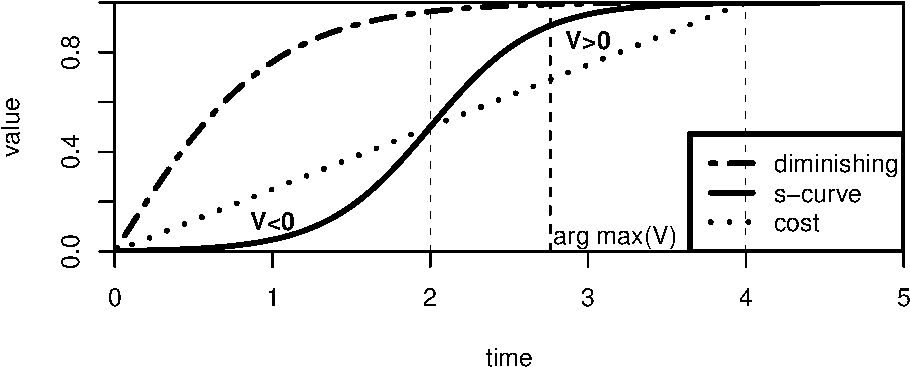
\includegraphics[scale=0.65]{s-curve.pdf}
\caption{Value of information curves} 
\label{fig:greedy-s-curve}
\end{figure} 

While it is often true that starting at
some point in time the returns never grow, until that point they can
alternate between increases and decreases. Figure~\ref{fig:greedy-s-curve}
shows a curve of diminishing returns (the
dashed curve), an s-curve (the solid curve), and the areas with
negative and positive values for the s-curved returns for a linear
time cost (the dotted straight line). Investments for the first two units
of time do not pay off, and the maximum return is achieved at
approximately $2.8$.

Experimental results show \cite{Zilberstein.sensing} that
sigmoid-shaped returns are not uncommon 
in search problems.  In such cases, an approach that can deal
with increasing returns must be used.
As the pure myopic scheme is too short-sighted in many cases,
some lookahead is needed, at increased computational cost.

Keeping the complexity manageable while overcoming the limitations of
the myopic algorithm is the basis for the \emph{semi-myopic} framework.
One might consider finding an optimal meta-level policy, but the
number of possible plans, even for discrete variables, is
super-exponential (and uncountably infinite for continuous variables),
which makes this approach infeasible.  In the semi-myopic schemes we
essentially assume (only for the sake of estimating VOI), that we need
to select meta-level actions offline. This makes the (simplified, but
incomplete) search space ``only'' exponential in the general case, and
polynomial in important, useful special cases.

Let, again, $M$ be the set of all possible meta-level actions, and
${\mathcal C}$ be a constraint over sets of actions from $M$. In the
semi-myopic framework, all possible subsets (batches) ${\mathcal B}$
of meta-level actions from $M$ that obey constraint ${\mathcal C}$ are
considered: for each such subset ${\mathcal B}$ a `batch' value of
information estimate is computed under the assumption that all
meta-level actions in ${\mathcal B}$ are made, followed by a decision.
Then, the batch ${\mathcal B}^*$ with the best
value estimate is chosen, and the meta-level action with the highest
VOI in ${\mathcal B}^*$ is performed.  The empty constraint $\mathcal
C$ results in the {\em exhaustive} scheme --- all possible action sets
are considered; this scheme has an exponential computation time, while
{\em still} not guaranteeing optimality (finding an
\emph{optimal} solution requires examination of all \emph{conditional plans}).
At the other extreme is the constraint where only singleton sets are
allowed. This extreme is tantamount to the myopic assumption.

In the presence of recurring meta-level actions, such as
noisy measurements, a useful compromise is the \textbf{blinkered
scheme}~\cite{TolpinShimony.blinkered}, which considers sets of
independent identical meta-level actions.  Although this scheme has a
computational overhead over the myopic one, the factor is only linear
in the budget.  The scheme selects a single meta-level action where
{\em some} number of the meta-level actions gains the greatest value
of information, and seems to be the simplest approximation that still
works for a wide range of conditions under realistic assumptions.
